\chapter{Codigos}\label{anexoA}
\thispagestyle{fancy}
\pagenumbering{arabic}\renewcommand{\thepage}{A.\arabic{page}}
    \section{}
        \subsection{}
        
        
        
\chapter{Desarrollo de formulas teóricas}\label{anexoB}
\thispagestyle{fancy}
\pagenumbering{arabic}\renewcommand{\thepage}{B.\arabic{page}}
    En este anexo se presentan el desarrollo detallado de las fórmulas presentadas en el capitulo \ref{CAP4} 
    
    
    \section{Metodología A}
        \subsection{Modelación Cinemática de Posición}
        
        \subsubsection{Nomenclatura y sistema de referencia local}
        En la siguiente ilustración se presenta la nomenclatura de los parámetros del robot delta simplificado, con su respectivo sistema de referencia local:
        
       \begin{figure}[h]
         \centering
          \subfloat[Gatito]{
           \label{f:Anexo_B_Metodo_A_Modelacion_Cinematica_Posicion_1}
            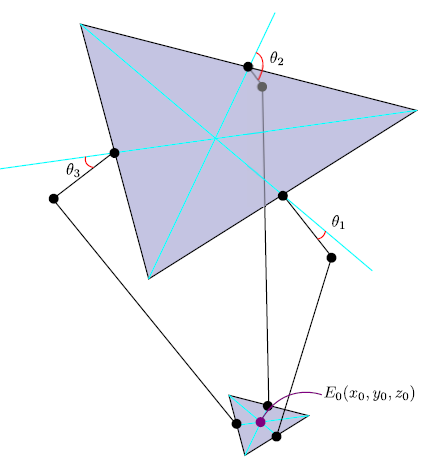
\includegraphics[width=0.5\textwidth]{Main/Chapter4/Images4/Metodo_A_Modelacion_Cinematica_Posicion_1.png}            }
          \subfloat[Tigre]{
           \label{f:Anexo_B_Metodo_A_Modelacion_Cinematica_Posicion_2}
            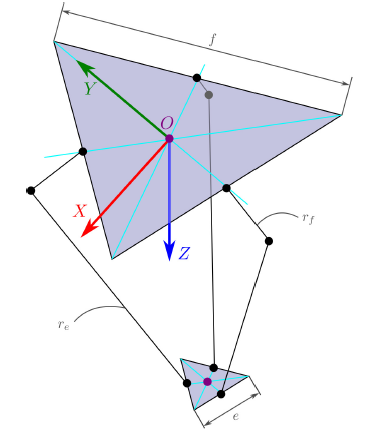
\includegraphics[width=0.5\textwidth]{Main/Chapter4/Images4/Metodo_A_Modelacion_Cinematica_Posicion_2.png}           }
         \caption{Múltiples imágenes}
         \label{f:Anexo_B_Metodo_A_Modelacion_Cinematica_Posicion_12}
        \end{figure}
        
        En la imagen se aprecia las piezas mecánicas básicas de un robot delta, tales como la  base fija, un efector móvil y 3 cadenas cinemáticas similares a un brazo robótico. Cada cadena esta compuestas por un actuador, que funciona como una junta revoluta, un brazo, una junta esférica que une el brazo con el antebrazo, un antebrazo y otra junta esférica que une al antebrazo con el efector. Los 3 actuadores están en los puntos medios de los lados del triangulo de la base fija.
        
        En la siguiente tabla se presenta la simbología de las magnitudes y vectores mas importantes para el desarrollo de la solución cinemática: 

        \begin{table}[H]
            \centering
            \begin{tabular}{>{\centering\arraybackslash}m{2cm} >{\arraybackslash}m{5cm} }
               Simbología  &  Descripción  \\\hline
               $f$  & Lado de base fija    \\\hline
               $e$  & Lado del efector    \\\hline
               $r_{f}$  & Longitud del brazo    \\\hline
               $r_{e}$  & Longitud del antebrazo    \\\hline
               $h_{f}$  & Segmento o altura perpendicular a un lado del triangulo hasta el centroide de la base fija.     \\\hline
               $h_{e}$  & Segmento o altura perpendicular a un lado del triangulo hasta el centroide del efector         \\\hline
               $\theta_{i}$  & Ángulo del actuador i    \\\hline
               $E_{0}(x_{0},y_{0},z_{0})$  & Coordenadas del centroide del efector   \\\hline
               $E_{i}$  & Coordenadas de las juntas esféricas que unen el antebrazo con el efector (punto medio del lado
               del triangulo que forma el efector) i=1,2,3.    \\\hline
               $F_{i}$  & Coordenadas de la posición del actuador i=1,2,3.    \\\hline
               $J_{i}$  & Coordenadas de las juntas esféricas que une el brazo unido al actuador i=1,2,3 con su antebrazo respectivo.    \\\hline
               $\overrightarrow{r_{f,l}}$  & Vector que representa la posición espacial del brazo que es movido por el actuador x. Vector que inicia en el actuador i=1,2,3 y termina en la junta que conecta brazo-antebrazo.     \\\hline
              $\overrightarrow{r_{e,l}}$  & Vector que representa la posición espacial del antebrazo unido al brazo que es movido por el actuador i. Vector que inicia desde la junta que conecta brazo-antebrazo y termina el punto medio de un borde del efector.    \\\hline
              $\overrightarrow{h_{f,l}}$  & Vector que representa la altura perpendicular triángulo formado por la base fija. Inicia en el centroide de la base fija hasta la posición del actuador i=1,2,3.    \\\hline
              $\overrightarrow{h_{e,l}}$  & Vector que representa la altura perpendicular triángulo formado por el efector. Inicia en el centroide del efecto hasta la posición de la junta esférica que una al antebrazo con el efector para cada cadena cinemática.    \\\hline
            \end{tabular}
            \caption{Referencias del dibujo}
            \label{tab:Anexo_B_my_label}
        \end{table}
        
        \begingroup
            \renewcommand{\arraystretch}{1.5}
            \begin{table}[H]
                \centering
                \begin{tabular}{|c|m{12cm}|}
                   \hline
                   \textbf{Simbología}  & \multicolumn{1}{c|}{\textbf{Descripción}}  \\\hline
                   $f$  & Lado de base fija                                         \\\hline
                   $e$  & Lado del efector                                          \\\hline
                   $r_{f}$  & Longitud del brazo                                    \\\hline
                   $r_{e}$  & Longitud del antebrazo                                \\\hline
                   $h_{f}$  & Segmento o altura perpendicular a un lado del triangulo hasta el centroide de la base fija.     \\\hline
                   $h_{e}$  & Segmento o altura perpendicular a un lado del triangulo hasta el centroide del efector         \\\hline
                   $\theta_{i}$  & Ángulo del actuador i    \\\hline
                   $E_{0}(x_{0},y_{0},z_{0})$  & Coordenadas del centroide del efector   \\\hline
                   $E_{i}$  & Coordenadas de las juntas esféricas que unen el antebrazo con el efector (punto medio del lado
                   del triangulo que forma el efector) i=1,2,3.    \\\hline
                   $F_{i}$  & Coordenadas de la posición del actuador i=1,2,3.    \\\hline
                   $J_{i}$  & Coordenadas de las juntas esféricas que une el brazo unido al actuador i=1,2,3 con su antebrazo respectivo.    \\\hline
                   $\overrightarrow{r_{f,l}}$  & Vector que representa la posición espacial del brazo que es movido por el actuador x. Vector que inicia en el actuador i=1,2,3 y termina en la junta que conecta brazo-antebrazo.     \\\hline
                  $\overrightarrow{r_{e,l}}$  & Vector que representa la posición espacial del antebrazo unido al brazo que es movido por el actuador i. Vector que inicia desde la junta que conecta brazo-antebrazo y termina el punto medio de un borde del efector.    \\\hline
                  $\overrightarrow{h_{f,l}}$  & Vector que representa la altura perpendicular triángulo formado por la base fija. Inicia en el centroide de la base fija hasta la posición del actuador i=1,2,3.    \\\hline
                  $\overrightarrow{h_{e,l}}$  & Vector que representa la altura perpendicular triángulo formado por el efector. Inicia en el centroide del efecto hasta la posición de la junta esférica que una al antebrazo con el efector para cada cadena cinemática.    \\\hline
                \end{tabular}
                \caption{Referencias del dibujo}
                \label{tab:Anexo_B_my_label2}
            \end{table}
        \endgroup
        
        \subsection{Modelación Cinemática de velocidad}
        
        
    \section{Metodología B}
        \subsection{Modelación Cinemática de posición}
        \subsection{Modelación Cinemática de velocidad}
        
        

            \paragraph{asd} 
                \subparagraph{asd}

        
\chapter{Planos}\label{anexoC}
\thispagestyle{fancy}
\pagenumbering{arabic}\renewcommand{\thepage}{B.\arabic{page}}
    \section{}
        \subsection{}